\chapter{Groups NET Distributed Implementation}
\label{ch:GroupsNet}

In D2D networks communication is established when a contact occurs, and the contacts are driven by human mobility. Therefore understanding human mobility and how people interact is a fundamental requirement to create suitable routing algorithms. Recent works have shown that the best routing solutions for D2D communication are those based on social context, mainly those that explore how people interact in groups or communities. In this chapter we propose a distributed implementation of Groups-NET, a forwarding algorithm based on group encounters \citep{nunes2016leveraging}. We propose an algorithm for group detection and tracking in a distributed environment and used it to implement Groups-NET. Through experiments with a real mobility trace containing 115 nodes we show that the solution achieves a good delivery ratio with an expressive lower network overhead when compared with the state-of-art BubbleRap algorithm.

<Write down the chapter structure when finished>
% This chapter is organized as follows. The section \ref{sec:groupsNet} details the original Groups NET implementation as is proposed in \cite{nunes2016leveraging}.
% The section \ref{sec:distributedGroupsNET} details the proposed distributed implementation inspired by the original Groups NET. This sectio is divided in two parts: in
% \ref{subsec:subsec:groupDetection} the grouping detection algorithm is detailed and in \ref{subsec:forwardingDistGroupsNET} the forwarding decision is also detailed.
% In section \ref{sec:GNExperiments}

\section{The Groups NET Algorithm}
\label{sec:groupsNet}

Groups-NET is a multi hop and multi copy forwarding algorithm for D2D networks that explores people group meetings to propagate content \citep{nunes2016leveraging}. A group is defined as a set of people that are placed near each other in a given time due to a common goal. For example, people working in the same company or students attending the same class. The algorithm is based on the idea that group encounters show some regularity along the time, because in general people have regular schedules and routines. Therefore we can explore group encounters to forward messages. In their previous work, \citet{groupMobility} proposed an algorithm for group detection and tracking, in which detected groups show encounters regularity along the time, mainly on daily and weekly basis.

This algorithm operates on contact traces and work as follows. First, the contact trace is split considering time windows of a predefined size. Contacts in each time window are used to create contact graphs, in which vertices denotes devices and edges denotes contacts in that time window. Then a sequence of graph contacts along the time is created, representing people contacts. For each of these graphs the clustering algorithm Clique Percolation \citep{derenyi2005clique} is applied to find clusters based on the contacts of that time interval. A cluster in a contact graph represents a group encounter in a that time window. In order to find groups that have encounters in different time windows the authors introduced the \textit{Group Correlation Coefficient} metric, which measures the similarity of two group captured in distinct contact graphs. This metric is defined as the number of intersection members of the two groups divided by the number of members of the union of the groups, therefore returning a value between 0 and 1. Groups detected in distinct time windows with \textit{Group Correlation Coefficient} greater or equals $0.5$ are considered as the same group with multiple encounters. So after applying the group detection algorithm we have a set of groups with its encounters along the analysed time.

Groups-NET forwards messages using the most probable group-to-group route based on the output of the group detection algorithm. Routes are computed using a graph in which groups are the vertices and there is an edge between each possible pair of groups. Edges are weighted considering the group correlation coefficient between the two groups and the probability of each group of encountering in the near future. The group correlation coefficient is expressed in equation \ref{eq:groupCorrelationCoefficient}. The probability of a group encountering is defined in equation \ref{eq:encounterProbability}, in which $TTL$ represents the time before a message is expired (we are interested in the probability of a group encountering before a given message has TTL expired) and $N$ represents the number of times a group has met considering the last $T$ hours. Based on these two values the edge weight is computed according to equation \ref{eq:edgeWeight}.

\begin{equation}
	\label{eq:groupCorrelationCoefficient}
	GC_{G_1G_2} = \frac{(G_1 \cap G_2)}{(G_1 \cup G_2)}
\end{equation}

\begin{equation}
	\label{eq:encounterProbability}
    P_G = 1 - e^{(-\frac{TTL * N}{T})}
\end{equation}

\begin{equation}
	\label{eq:edgeWeight}
    E_{G_1G_2} = -\log(GC_{G_1G_2} * P_{G1} * P_{G2})
\end{equation}

With the groups graph defined it is possible to find the route to forward a message. Given a message with defined source and destination nodes, we compute shortest paths for each pair of groups $(G_s \rightarrow G_d)$, in which $G_s$ is a group that the source is present and $G_d$ is a group that the destination node is present. From this list of paths the shortest one is chosen as the most probable group-to-group path. The message is then forwarded upon a contact if the other node is present in one of the groups of the chosen path. Thought experiments, the authors show that Groups-NET outperforms Bubble-Rap in terms of network overhead. However, this solution relies on the global network knowledge to detect and track groups, which is unfeasible in real scenarios. In the next section we go over a proposed solution to detect groups in a distributed environment. We then use this definition later combined with the original forwarding decision mechanism of Groups-NET to build the distributed solution.


\section{Mobile Group Detection}
\label{sec:distributedGroupsNET}

The mobile group detection algorithm proposed here is derived from the ideas presented in \citep{groupMobility}. In the original proposal the authors use a approach to detect groups based on global network knowledge. They basically build a contact graph considering a predefined time interval, and for each graph is used the Clique Percolation community detection algorithm. Each community detected by the algorithm is considered a group meeting in that time window. Then
a metric called \textit{Group Correlation Coefficient} is used to detect instances of the same group across multiple time windows. With this approach the authors show that groups usually have regular encounters along the time (specially in daily and weekly basis). But they also discuss that the detection approach is unfeasible for a distributed environment, because it assumes a global network knowledge.

However, authors also discuss that implementing a distributed solution should be a simple task, because in the local scope nodes can use neighborhood discover strategies and process regular neighbors encounters to decide their group encounters. In this work we expanded this idea to build a distributed solution for group detection. It is composed of four processes that are executed concurrently by each node using basically neighborhood inspection.

The first process is the \textbf{device's local group detection}. This process is responsible of inspecting a node's local contacts and decide when a group meeting happens. The algorithm is very simple. Each node keeps two lists of devices. The first is the \textit{friends list} (\textit{FL}) that keeps track of current nodes considered as friends, i.e, members of a recent group encounter. The second list is the \textit{strangers list} (\textit{SL}), that keeps track of recent nodes' contacts that are not yet considered as friends (random contacts, for example). Each entry in these lists have a contact counter that keeps track of consecutive contacts, and also have a inactive counter that keeps track of consecutive periods of time without contact with that node. Each node inspects its neighborhood at each predefined \textit{time interval} and based on current neighbors it updates its friends and strangers list. This update is based on two predefined parameters: the \textit{friend threshold} and \textit{inactive threshold}. Based on these definitions this process is executed as follows:

\begin{itemize}
	\item At each time interval each node collects its current neighbors.
	\item Each node use its current neighbors to update the counters of friends list members. Current neighbors that are present in the friends list have their contact counters incremented by one and its inactive counter set to zero. Current friends that are not a current neighbor have their contact counters set to zero and their inactive counter incremented by one.
	\item A similar update is made to strangers list. Current neighbors that are present in the strangers list have their contact counter incremented by one and their inactive counter set to zero. If a stranger contact counter reaches the defined \textit{friend threshold}, the stranger is promoted to a friend and moved to the friends list. Current strangers that are not a current neighbor have its inactive counter incremented by one and its contact counter set to zero. If a stranger inactive counter reaches a \textit{inactive threshold} the node is removed from strangers list.
	\item Current neighbors that are not in friends and strangers list are added in the strangers list with their contact counter set to one and inactive counter set to zero.
	\item As a final step, the number of inactive nodes in the friends list that are checked. A node is considered inactive when the inactive counter reaches the \textit{inactive threshold}. If more than 50 percent of the nodes in the friends list are inactive, the friend list is archived and considered as a group meeting that happened in the past. When this happens, both friends and strangers list are clear and the algorithm is restarted.
\end{itemize}

In the end this algorithm creates a list of local detected group meetings. This list is used by the \textbf{local group combination} process to detect instances of the same group with multiple encounters along the time. In this process each mobile device analyzes groups discovered by the previous process to define groups that have multiple encounters along the time. The algorithm is based on the \textit{Group Correlation Coefficient} metric that measures the proportion of nodes shared between two sets. Each node keeps a list of \textit{combined groups}, that keeps track of current known groups with multiple encounters along the time. For each local group detected in the previous process, it checks if there is a combined group with \textit{Group Correlation Coefficient} greater or equals 0.5. If there is, the local group is merged into the combined group adding its members to it and registering a new encounter. If there isn't, a new combined group is initialized with the local group data.

The combined groups generated are then used by the \textbf{neighborhood inspection} process to compose the final groups considered in the forwarding algorithm. This process is responsible of at each considered time interval collecting a node's neighbors combined groups. The collected groups are then merged with the local combined groups using the same approach described previously, in which groups that have correlation coefficient greater of equals 0.5 are merged. The purpose of this process is to expand the nodes global knowledge. The list of combined groups are then used for the \textbf{groups graph creation} process to create the graph used by the forwarding decision mechanism of Groups-NET. The next section describe the experiments used to validate the proposed solution.

\section{Simulation Methodology}
\label{sec:GNExperiments}

In order to validate the proposed solution we executed some message forwarding simulations comparing the performance of distributed Groups-NET against the performance of the distributed version of Bubble Rap \citep{hui2011bubble} based on the distributed community detection algorithm presented by \citet{hui2007distributed}. Both forwarding algorithms were implemented\footnote{The code is available at https://github.com/micdoug/the-one/tree/groups-net.} as an extension to the ONE (Opportunistic Network) simulator. The distributed group detection algorithm presented in the previous section was implemented as an external script\footnote{The code is available at https://github.com/micdoug/mgb.} that generates the group graph structure and give as input to the ONE simulator. The reason of this is that adding parallelism in the ONE simulator would require modification on the core of the simulator, and without parallelism the simulation performance highly degrades due to the massive groups graph manipulation requirement.

We have used for simulation the NCCU mobility trace \citep{tsai2015nccu}, a real-world dataset that monitors the mobility of 115 students inside a campus for 15 days. We considered the entire trace duration to run the group detection algorithm for Groups-NET and community detection algorithm for BubbleRap. And we used the second week to simulate message forwarding. We decided to use the 15 days for the group detection algorithm to capture the weekly regularity of group encounters, that is presented in the results of next section. Another reason is that the to compute the groups graph edges weight we need to consider a message TTL and the number of encounters in the last $T$ hours, so we defined $T$ as the first seven days and the message TTL as the next 7 days.

To compare the two forwarding algorithms we evaluated the delivery ratio and network overhead. The delivery ratio evaluates the percentage of delivered messages along the time. The network overhead evaluates the number of retransmissions per created message in the network, i.e., the number of D2D transmissions that each algorithm performs along the time normalized by the number of created messages. Forwarding algorithms seek for the highest delivery ratio with the lowest possible network overhead. Successfully delivered messages are those which the base station will not need to deliver itself, thus using less bandwidth. A high number of message re-transmissions (high overhead) may negatively impact the users' experience by, for example, increasing devices' energy expenditure.

The parameters used for simulation are summarized in table \ref{tab:groupsNetParameters}. In the next section we present the results of group detection and message forwarding using the proposed solution.

\begin{table}[H]
	\centering
	\caption{Simulation Parameters}
	\label{tab:groupsNetParameters}
	\begin{tabular}{|l|l|}
	\hline
	\textbf{Parameter}  & \textbf{Value} \\ \hline
	friend threshold    & 10             \\ \hline
	inactive threshold  & 10             \\ \hline
	scan time interval  & 60 seconds     \\ \hline
	message TTL         & 7 days         \\ \hline
	T (past encounters) & 7 days         \\ \hline
	number of messages  & 5000           \\ \hline
	\end{tabular}
	\end{table}

\section{Results}
\label{sec:GNResults}

We executed the mobile group detection on NCCU trace using using the parameters presented in table \ref{tab:groupsNetParameters}. Other combination of parameters were used, however this one has showed the same behavior of the centralized version in terms of group reencounters distribution. The figure \ref{fig:groupReencounters} shows the distribution of group reencounters. The group reencounters distribution shows spikes on intervals of 24 hours (dotted orange lines) and 7 days (green dotted lines). So this shows that the groups collected from the distributed algorithm captures similar characteristics of the centralized version. After validating this, we used these detected groups to run the message forwarding simulation.

Figure \ref{fig:groupSimulationResults} shows the message forwarding simulation results. Groups-NET has achieved a lower message delivery ratio, about 15 percent at the end of the simulation when comparing it with Bubble Rap. However the message overhead achieved by Groups-NET is more than 4 times lower than Bubble Rap at the end of simulation, a value expressively better. It is also important to notice that the message overhead ratio of Groups-NET have established from the second day of simulation until the end, in contrast Bubble Rap number of copies continues to increase.

\begin{figure}
	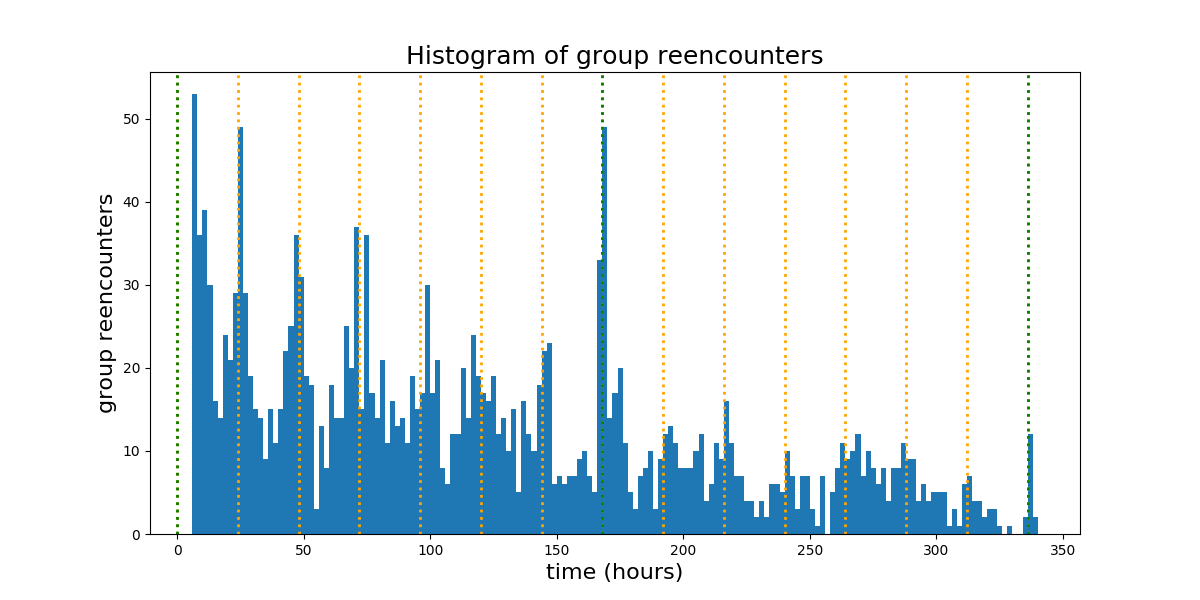
\includegraphics[width=\linewidth]{imgs/groups-net/group-reencounters.png}
    \caption{Group reencounters distribution results of the distributed group detection algorithm}
    \label{fig:groupReencounters}
\end{figure}

\begin{figure}
    \begin{subfigure}[b]{0.5\columnwidth}
        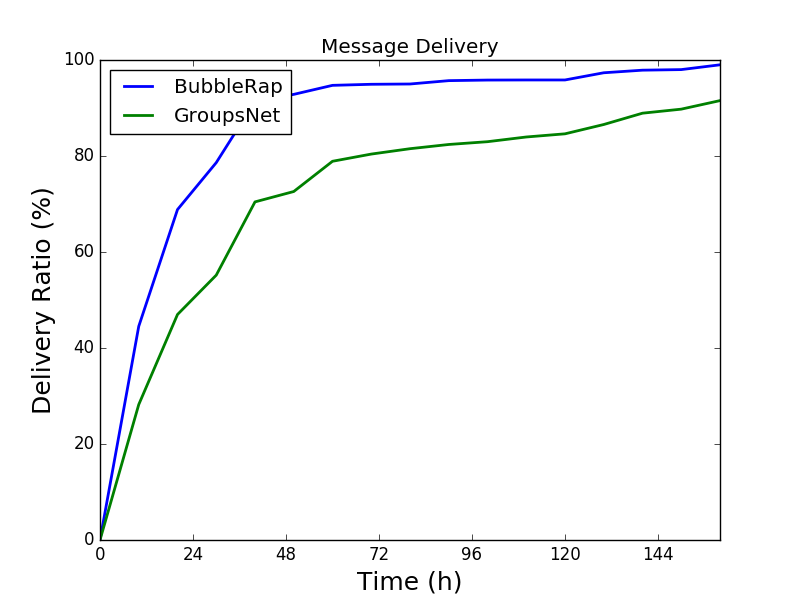
\includegraphics[width=\linewidth]{imgs/groups-net/GroupsNet-delivery.png}
        \caption{Delivery ratio results}
        \label{fig:groupMessageDelivery}
    \end{subfigure}
    \hfill %%
    \begin{subfigure}[b]{0.5\columnwidth}
        \includegraphics[width=\linewidth]{imgs/groups-net/GroupsNET-overhead.png}
        \caption{Message overhead results}
        \label{fig:groupOverhead}
    \end{subfigure}

    \caption{Comparison of distributed Groups-NET and BubbleRap on NCCU trace}
    \label{fig:groupSimulationResults}
\end{figure}


\section{Conclusion}
\label{sec:GNConclusion}




